\documentclass[12pt,ngerman,parskip=half]{scrartcl}

\usepackage{babel}
\usepackage{tikz}
\usetikzlibrary{shapes}
% https://tikz.dev/tikz-arrows
\usetikzlibrary {arrows.meta} 

\usepackage{blindtext}

\begin{document}

\blindtext


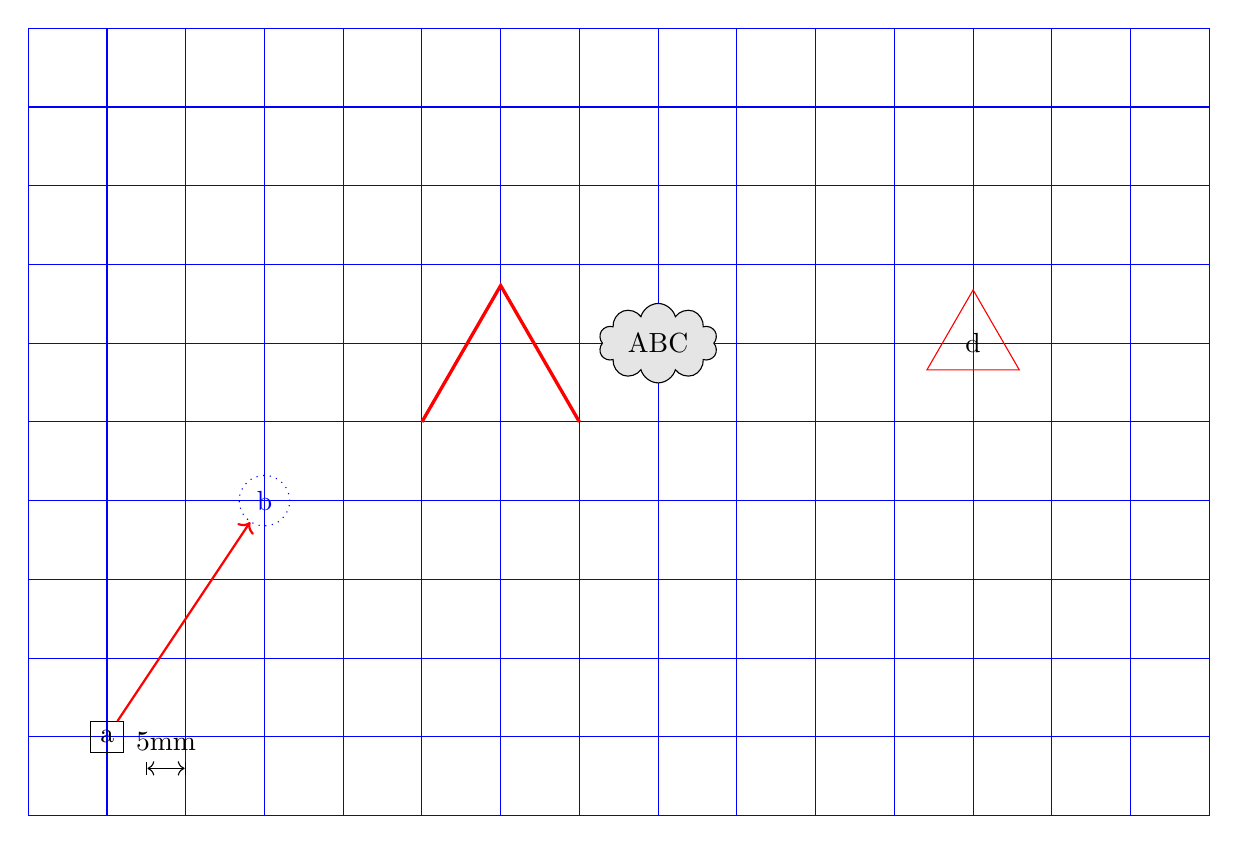
\begin{tikzpicture} 
\draw [step=1cm,blue,thin] (0,0) grid (15,10);
\draw[red,very thick] (5,5) -- ++(60:2)  -- ++(-60:2);

\node[rectangle,draw] (a) at (1,1){a};
\node[circle,draw,blue,dotted] (b) at (3,4){b};

\draw [->,red,thick] (a) -- (b);

\node[draw=red,regular polygon, regular polygon sides=3] (c) at (12,6){d};

\draw [|<->|] (1.5,.6) -- node[above=1mm] {5mm} (2,.6);

\node[cloud, draw, fill=gray!20, aspect=2] at (8,6) {ABC};

\end{tikzpicture}

\blindtext


\end{document}